\documentclass[tikz,border=12pt]{standalone}
\usepackage{tikz}
\usepackage{amsmath}
\usepackage{amssymb}
\usetikzlibrary{
  shapes.geometric,
  shapes.multipart,
  arrows.meta,
  positioning,
  fit,
  backgrounds,
  shadows.blur,
  calc,
  matrix,
  decorations.pathreplacing,
  decorations.markings
}

%% ===== COLOR PALETTE =====
\definecolor{CPurple50}{HTML}{EEEDFE}
\definecolor{CPurple400}{HTML}{7D77D4}
\definecolor{CPurple600}{HTML}{534AB7}
\definecolor{CPurple800}{HTML}{3C3489}
\definecolor{CTeal50}{HTML}{E1F5EE}
\definecolor{CTeal400}{HTML}{3CB88A}
\definecolor{CTeal600}{HTML}{0F6E56}
\definecolor{CTeal800}{HTML}{085041}
\definecolor{CAmber50}{HTML}{FAEEDA}
\definecolor{CAmber400}{HTML}{D48B2E}
\definecolor{CAmber600}{HTML}{854F0B}
\definecolor{CCoral50}{HTML}{FAECE7}
\definecolor{CCoral400}{HTML}{D85A30}
\definecolor{CCoral600}{HTML}{993C1D}
\definecolor{CRed50}{HTML}{FCEBEB}
\definecolor{CRed400}{HTML}{C94040}
\definecolor{CRed600}{HTML}{A32D2D}
\definecolor{CGray50}{HTML}{F5F4F0}
\definecolor{CGray200}{HTML}{D8D5C8}
\definecolor{CGray500}{HTML}{888780}
\definecolor{CGray800}{HTML}{444441}
\definecolor{CBlue50}{HTML}{E6F1FB}
\definecolor{CBlue600}{HTML}{185FA5}
\definecolor{CWhite}{HTML}{FFFFFF}

%% ===== TIKZ STYLES =====
\tikzset{
  %% --- ERD boxes ---
  erd header/.style={
    rectangle, draw, line width=0.8pt,
    rounded corners=4pt,
    text width=4.0cm, align=center,
    font=\small\bfseries,
    inner sep=6pt, minimum height=0.8cm
  },
  erd field/.style={
    rectangle, draw=CGray200, line width=0.4pt,
    text width=3.8cm, align=flush left,
    font=\scriptsize,
    inner sep=4pt, minimum height=0.52cm
  },
  erd field vuln/.style={erd field, fill=CCoral50},
  erd field safe/.style={erd field, fill=CTeal50},
  erd field normal/.style={erd field, fill=CWhite},
  erd field gray/.style={erd field, fill=CGray50},
  %% --- Arrows ---
  arr/.style={
    -Stealth, line width=0.9pt, color=CGray500
  },
  arr red/.style={
    -Stealth, line width=1.0pt, color=CRed400,
    dashed
  },
  arr teal/.style={
    -Stealth, line width=1.0pt, color=CTeal600
  },
  arr purple/.style={
    -Stealth, line width=1.0pt, color=CPurple600
  },
  arr amber/.style={
    -Stealth, line width=1.0pt, color=CAmber600
  },
  %% --- Labels ---
  edge label/.style={
    font=\scriptsize, text=CGray500,
    fill=CWhite, inner sep=1pt
  },
  title main/.style={font=\large\bfseries, text=CGray800},
  title sub/.style={font=\small, text=CGray500}
}

\begin{document}
%% ===========================================================
%% DIAGRAM 2: SƠ ĐỒ QUAN HỆ (ENTITY RELATIONSHIP)
%% 3 struct: GiangVien, LopHocPhan, Config
%% ===========================================================
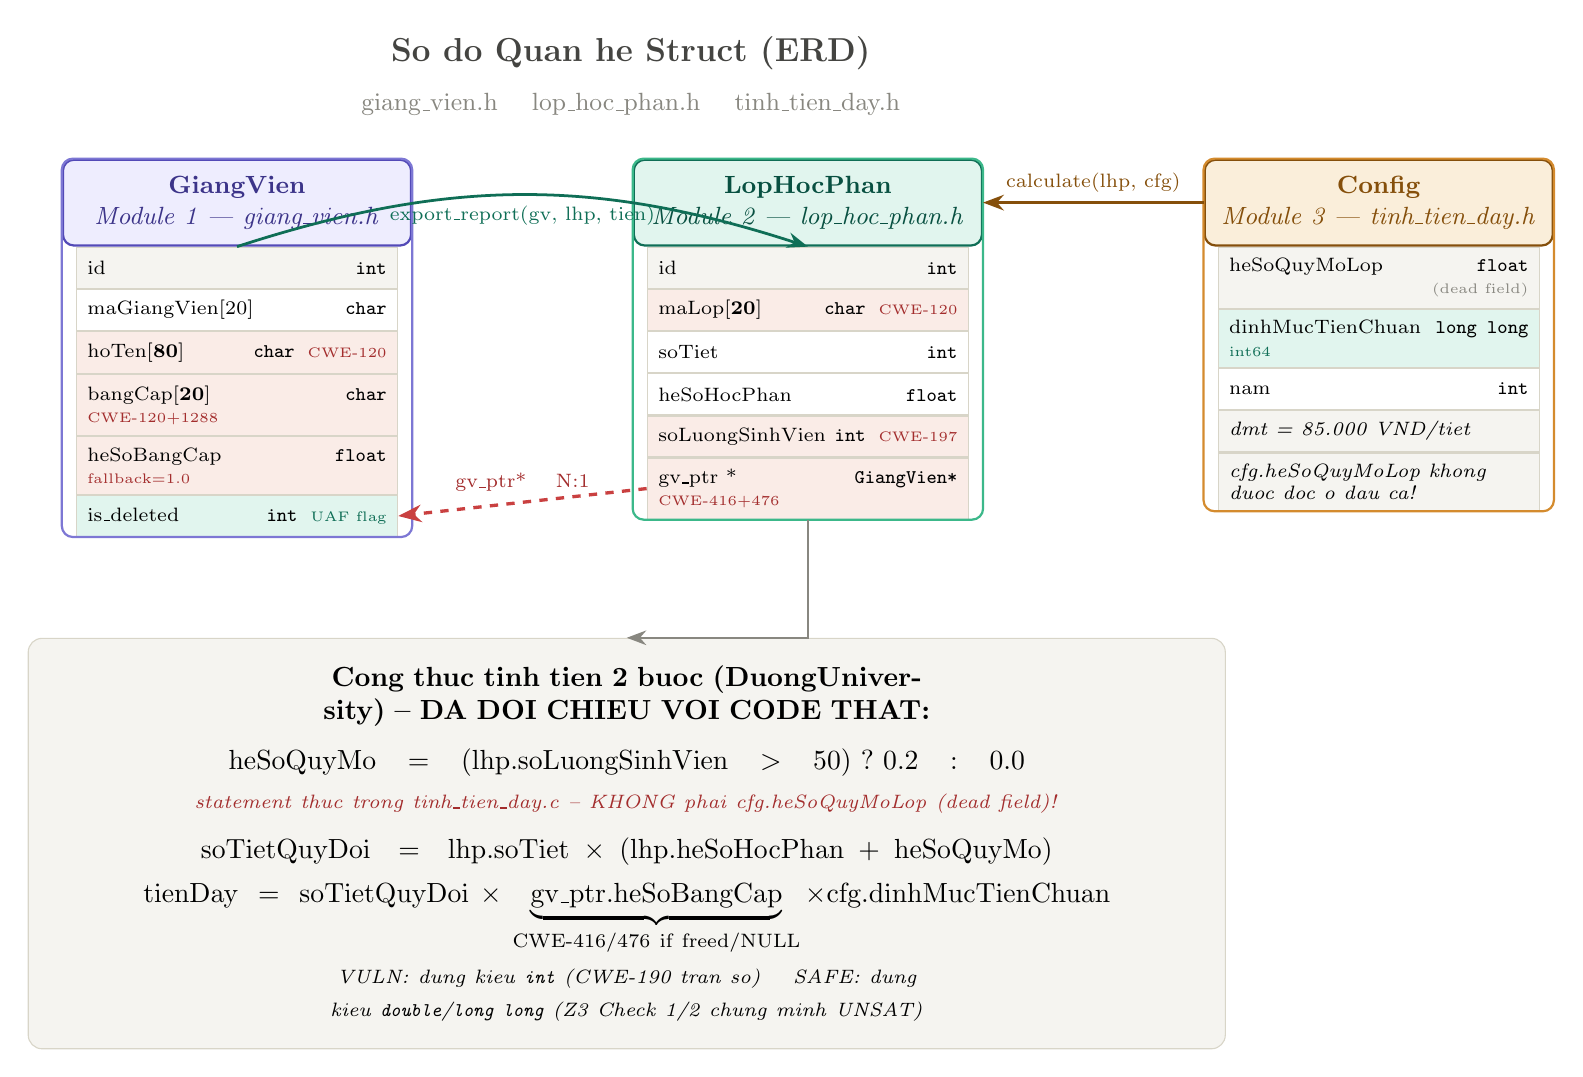
\begin{tikzpicture}

\node[title main] (T2) at (0,0)
  {So do Quan he Struct (ERD)};
\node[title sub, below=0.05cm of T2]
  {giang\_vien.h \quad lop\_hoc\_phan.h \quad tinh\_tien\_day.h};

%% ===== GiangVien =====
\node[erd header, fill=CPurple50, draw=CPurple600, text=CPurple800,
  below=1.0cm of T2, xshift=-5.0cm] (GVH)
  {GiangVien\\\small\normalfont\textit{Module 1 --- giang\_vien.h}};

\node[erd field gray,   below=0pt of GVH] (gv1) {id \hfill \texttt{int}};
\node[erd field normal, below=0pt of gv1] (gv2) {maGiangVien[20] \hfill \texttt{char}};
\node[erd field vuln,   below=0pt of gv2] (gv3)
  {hoTen[\textbf{80}] \hfill \texttt{char}
   \hspace{2pt}\textcolor{CRed600}{\tiny CWE-120}};
\node[erd field vuln,   below=0pt of gv3] (gv4)
  {bangCap[\textbf{20}] \hfill \texttt{char}
   \hspace{2pt}\textcolor{CRed600}{\tiny CWE-120+1288}};
\node[erd field vuln, below=0pt of gv4] (gv5)
  {heSoBangCap \hfill \texttt{float}
   \hspace{2pt}\textcolor{CRed600}{\tiny fallback=1.0}};
\node[erd field safe,   below=0pt of gv5] (gv6)
  {is\_deleted \hfill \texttt{int}
   \hspace{2pt}\textcolor{CTeal600}{\tiny UAF flag}};

\node[draw=CPurple400, line width=0.8pt, rounded corners=4pt,
  fit=(GVH)(gv1)(gv2)(gv3)(gv4)(gv5)(gv6),
  inner sep=0pt] (GV box) {};

%% ===== LopHocPhan =====
\node[erd header, fill=CTeal50, draw=CTeal600, text=CTeal800,
  right=2.8cm of GVH] (LHPH)
  {LopHocPhan\\\small\normalfont\textit{Module 2 --- lop\_hoc\_phan.h}};

\node[erd field gray,   below=0pt of LHPH] (lhp1) {id \hfill \texttt{int}};
\node[erd field vuln,   below=0pt of lhp1] (lhp2)
  {maLop[\textbf{20}] \hfill \texttt{char}
   \hspace{2pt}\textcolor{CRed600}{\tiny CWE-120}};
\node[erd field normal, below=0pt of lhp2] (lhp3)
  {soTiet \hfill \texttt{int}};
\node[erd field normal, below=0pt of lhp3] (lhp4)
  {heSoHocPhan \hfill \texttt{float}};
\node[erd field vuln, below=0pt of lhp4] (lhp5)
  {soLuongSinhVien \hfill \texttt{int}
   \hspace{2pt}\textcolor{CRed600}{\tiny CWE-197}};
\node[erd field vuln,   below=0pt of lhp5] (lhp6)
  {gv\_ptr * \hfill \texttt{GiangVien*}
   \hspace{2pt}\textcolor{CRed600}{\tiny CWE-416+476}};

\node[draw=CTeal400, line width=0.8pt, rounded corners=4pt,
  fit=(LHPH)(lhp1)(lhp2)(lhp3)(lhp4)(lhp5)(lhp6),
  inner sep=0pt] (LHP box) {};

%% ===== Config =====
\node[erd header, fill=CAmber50, draw=CAmber600, text=CAmber600,
  right=2.8cm of LHPH] (CFGH)
  {Config\\\small\normalfont\textit{Module 3 --- tinh\_tien\_day.h}};

\node[erd field gray, below=0pt of CFGH] (cfg1)
  {heSoQuyMoLop \hfill \texttt{float}\\
   \hfill\textcolor{CGray500}{\tiny (dead field)}};
\node[erd field safe,   below=0pt of cfg1] (cfg2)
  {dinhMucTienChuan \hfill \texttt{long long}
   \hspace{2pt}\textcolor{CTeal600}{\tiny int64}};
\node[erd field normal, below=0pt of cfg2] (cfg3)
  {nam \hfill \texttt{int}};
\node[erd field gray, below=0pt of cfg3] (cfg4)
  {\textit{dmt = 85.000 VND/tiet}};
\node[erd field gray, below=0pt of cfg4] (cfg5)
  {\textit{\scriptsize cfg.heSoQuyMoLop khong duoc doc o dau ca!}};

\node[draw=CAmber400, line width=0.8pt, rounded corners=4pt,
  fit=(CFGH)(cfg1)(cfg2)(cfg3)(cfg4)(cfg5),
  inner sep=0pt] (CFG box) {};

%% ===== RELATIONSHIPS =====
%% gv_ptr: LopHocPhan (N) -> GiangVien (1)
\draw[arr red, line width=1.2pt]
  (lhp6.west) --
  node[above, font=\scriptsize, text=CRed600]
    {gv\_ptr* \quad N:1}
  (gv6.east);

%% calculate() uses LHP + CFG
\draw[arr amber]
  (CFGH.west) --
  node[above, font=\scriptsize, text=CAmber600]
    {calculate(lhp, cfg)}
  (LHPH.east);

%% export() uses GV + LHP
\draw[arr teal, bend left=18]
  (GVH.south) to
  node[below, font=\scriptsize, text=CTeal600]
    {export\_report(gv, lhp, tien)}
  (LHPH.south);

%% ===== FORMULA BOX =====
%% DA SUA: cong thuc THAT dung heSoQuyMo suy tu lhp.soLuongSinhVien (statement
%% ro rang), KHONG PHAI cfg.heSoQuyMoLop (dead field, xem ghi chu CFG o tren) --
%% day la loi mo hinh-code that da tim thay va sua o Check 1/2 (Chuong 3).
\node[draw=CGray200, fill=CGray50, rounded corners=5pt,
  text width=14.5cm, align=center, inner sep=10pt,
  below=1.5cm of lhp6, xshift=-2.3cm] (formula)
{
  \textbf{Cong thuc tinh tien 2 buoc (DuongUniversity) -- DA DOI CHIEU VOI CODE THAT:}\\[6pt]
  $\text{heSoQuyMo} = (\text{lhp.soLuongSinhVien} > 50)\ ?\ 0.2 : 0.0$\\[2pt]
  \textcolor{CRed600}{\scriptsize\textit{statement thuc trong tinh\_tien\_day.c -- KHONG phai cfg.heSoQuyMoLop (dead field)!}}\\[6pt]
  $\text{soTietQuyDoi} = \text{lhp.soTiet}
    \times (\text{lhp.heSoHocPhan} + \text{heSoQuyMo})$\\[4pt]
  $\text{tienDay} = \text{soTietQuyDoi}
    \times \underbrace{\text{gv\_ptr.heSoBangCap}}_{\text{CWE-416/476 if freed/NULL}}
    \times \text{cfg.dinhMucTienChuan}$\\[4pt]
  \textit{\scriptsize VULN: dung kieu \texttt{int} (CWE-190 tran so)
    \quad SAFE: dung kieu \texttt{double}/\texttt{long long} (Z3 Check 1/2 chung minh UNSAT)}
};

\draw[arr] (lhp6.south) |- (formula.north);

\end{tikzpicture}
\end{document}
